\documentclass[11pt]{article}

\usepackage{pablo}
\usepackage{pgfplots}
\usepackage{multicol}
\usepackage{tkz-tab}
\usepackage{numprint}
\usepackage[a5paper,margin=1.7cm]{geometry}

\pagestyle{empty}
\begin{document}

\begin{center}
  {\large
    Correction de DM

    \textsc{Fonctions affines --- Inéquations}
  }
\end{center}

\begin{exercice}[Fonctions affines]~
  \begin{enumerate}[(1)]
    \item \emph{Calculer l'équation de la droite $\cal D$ passant par les points $A(\frac{1}{3}; 2)$ et $B(1; \frac{2}{3})$.}
      On cherche une équation de la forme $y=ax+b$. On sait que $a=\frac{y_B-y_A}{x_B-x_A}=\frac{\frac{2}{3}-2}{1-\frac{1}{3}}=-2$. Nous avons maintenant une équation de la forme $y=-2x-b$. Reste à calculer $b$. Le point $A$ appartient à la droite, donc ses coordonnées vérifient l'équation de la droite, donc $y_A=-2x_A+b$, c'est-à-dire $2=-2\times\frac{1}{3}+b$. C'est une équation du premier degré, la solution est $b=\frac{8}{3}$. L'équation de la droite est donc $y=-2x+\frac{8}{3}$.
    \item \emph{Dans un repère orthonormé, placer les points $A$, $B$, et tracer la droite $\cal D$. Vérifier la cohérence du tracé.}
      \begin{multicols}{2}
      \begin{center}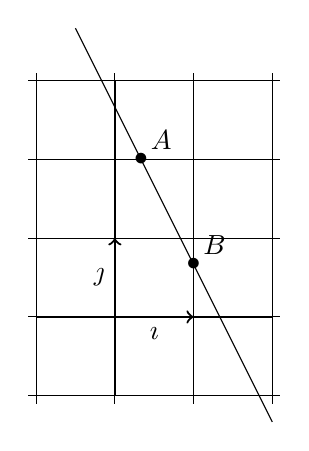
\begin{tikzpicture}
        \draw(-1.1,-1.1) grid (2.1,3.1);
        \draw(1/3,2) node{$\bullet$} node[above right]{$A$};
        \draw(1,2/3) node{$\bullet$} node[above right]{$B$};
        \draw(-0.5,11/3) -- (2,-4/3);
        \draw[thick](-1,0)--(2,0);
        \draw[thick](0,-1)--(0,3);
        \draw[thick][->](0,0)->(1,0) node[midway,below]{$\vecteur\imath$};
        \draw[thick][->](0,0)->(0,1) node[midway,left]{$\vecteur\jmath$};
      \end{tikzpicture}\end{center}
      Vérifications possibles :
      \begin{itemize}
      \item Lecture graphique du coefficient directeur.
      \item Lecture graphique de l'ordonnée à l'origine.
      \item Placer un troisième point, et vérifier qu'il appartient bien à la droite.
    \end{itemize}
  \end{multicols}
  \end{enumerate}
\end{exercice}

\begin{exercice}[Problème]~

  \begin{multicols}{2}
  \begin{center}
    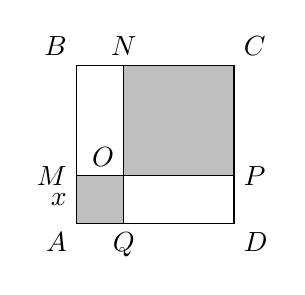
\begin{tikzpicture}[scale=2]
      \draw (0,0) rectangle (1,1);
      \draw [fill=lightgray] (0,0) rectangle (0.3,0.3);
      \draw [fill=lightgray] (1,1) rectangle (0.3,0.3);
      \node[below left] at (0,0) {$A$};
      \node[above left] at (0,1) {$B$};
      \node[above right] at (1,1) {$C$};
      \node[below right] at (1,0) {$D$};
      \node[left] at (0,0.3) {$M$};
      \node[right] at (1,0.3) {$P$};
      \node[above] at (0.3,1) {$N$};
      \node[below] at (0.3,0) {$Q$};
      \node[above left] at (0.3,0.3) {$O$};
      \draw (0,0) -- (0,0.3) node[midway,left]{$x$};
    \end{tikzpicture}
  \end{center}

    \begin{enumerate}[(1)]
      \item \emph{Quelles sont les valeurs possibles pour $x$ ?}
        
        $M$ est un point du segment $[AB]$, de longueur 6. Donc $x\in[0;6]$.
    \end{enumerate}
  \end{multicols}
    \begin{enumerate}[(1)]
        \setcounter{enumi}{1}
      \item \emph{Montrer que ${\cal A}(x)=x^2+(6-x)^2$.}
        
        $OMAQ$ et $NCPO$ sont des carrés, d'aires respectives $x^2$ et $(6-x)^2$. L'aire grisée est la somme des deux, d'où la formule.
      \item \begin{enumerate}[(a)]
          \item \emph{Montrer que le problème revient à résoudre l'inéquation $2x^2-12x+16\geq0$.}
            
            On cherche les valeurs de $x$ pour lesquelles ${\cal A}(x)$ est supérieure à \numprint[cm\up{2}]{20}, c'est-à-dire ${\cal A}(x)\geq20$.  
            Donc :\\
            $x^2+(6-x)^2\geq20$\\
            $x^2+36-12x+x^2\geq20$\\
            $2x^2-12x+36-20\geq20$\\
            $2x^2-12x+16\geq0$.
          \item \emph{Montrer que $2x^2-12x+16=(2x-4)(x-4)$.}

            Il suffit de développer le second membre :\\ $(2x-4)(x-4)=2x^2+2x\times(-4)-4x+16$

            \hspace{7em}$=2x^2-12x+16$.
          \item \emph{Résoudre $(2x-4)(x-4)\geq0$.}
            
            C'est une équation produit, qui se résoud avec un tableau de signes. Commençons par résoudre les deux équations :
            \begin{itemize}
              \item[$\bullet$] $2x-4\geq0$ si $x\geq2$ ;
              \item[$\bullet$] $x-4\geq0$ si $x\geq4$.
            \end{itemize}
            Le tableau de signes est alors le suivant :

          \hspace{-2em}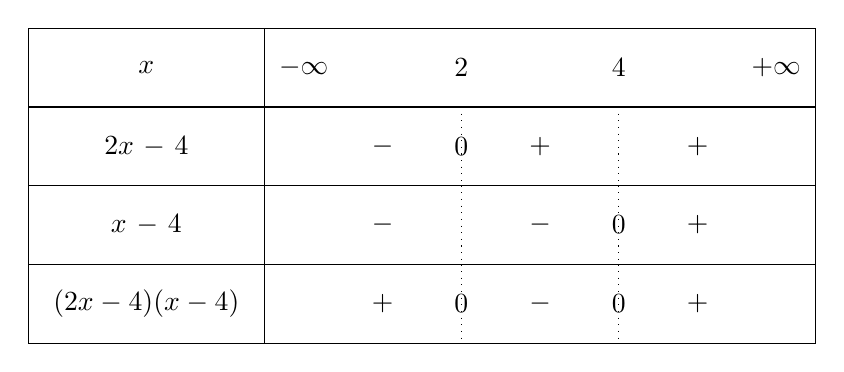
\begin{tikzpicture}
            \tkzTabInit[lgt=3,espcl=2]
            {$x$ /1,
              $2x-4$ /1,
            $x-4$ /1,
            $(2x-4)(x-4)$ /1}
            {$-\infty$,$2$,$4$,$+\infty$}%
            \tkzTabLine { ,-,z,+,t,+ }
            \tkzTabLine { ,-,t,-,z,+ }
            \tkzTabLine { ,+,z,-,z,+ }
          \end{tikzpicture}

      \noindent Et on lit dans la dernières ligne que les solutions sont :
  
  $x\in]-\infty;2]\cup[4;\infty[$.
          \end{enumerate}
        \item \emph{Répondre à la question posée au départ.}
          
          Nous avons dit au départ que $x\in[0;6]$. Donc, en combinant cette information avec la précédente, nous trouvons $x\in[0;2]\cup[4;6]$.
    \end{enumerate}
\end{exercice}

\end{document}
